


\begin{frame}{Contents}
  \begin{center}
   \Large Part 5: ViennaFEM
  \end{center}
\end{frame}


\begin{frame}{Simulation Flow}
  \begin{center}
   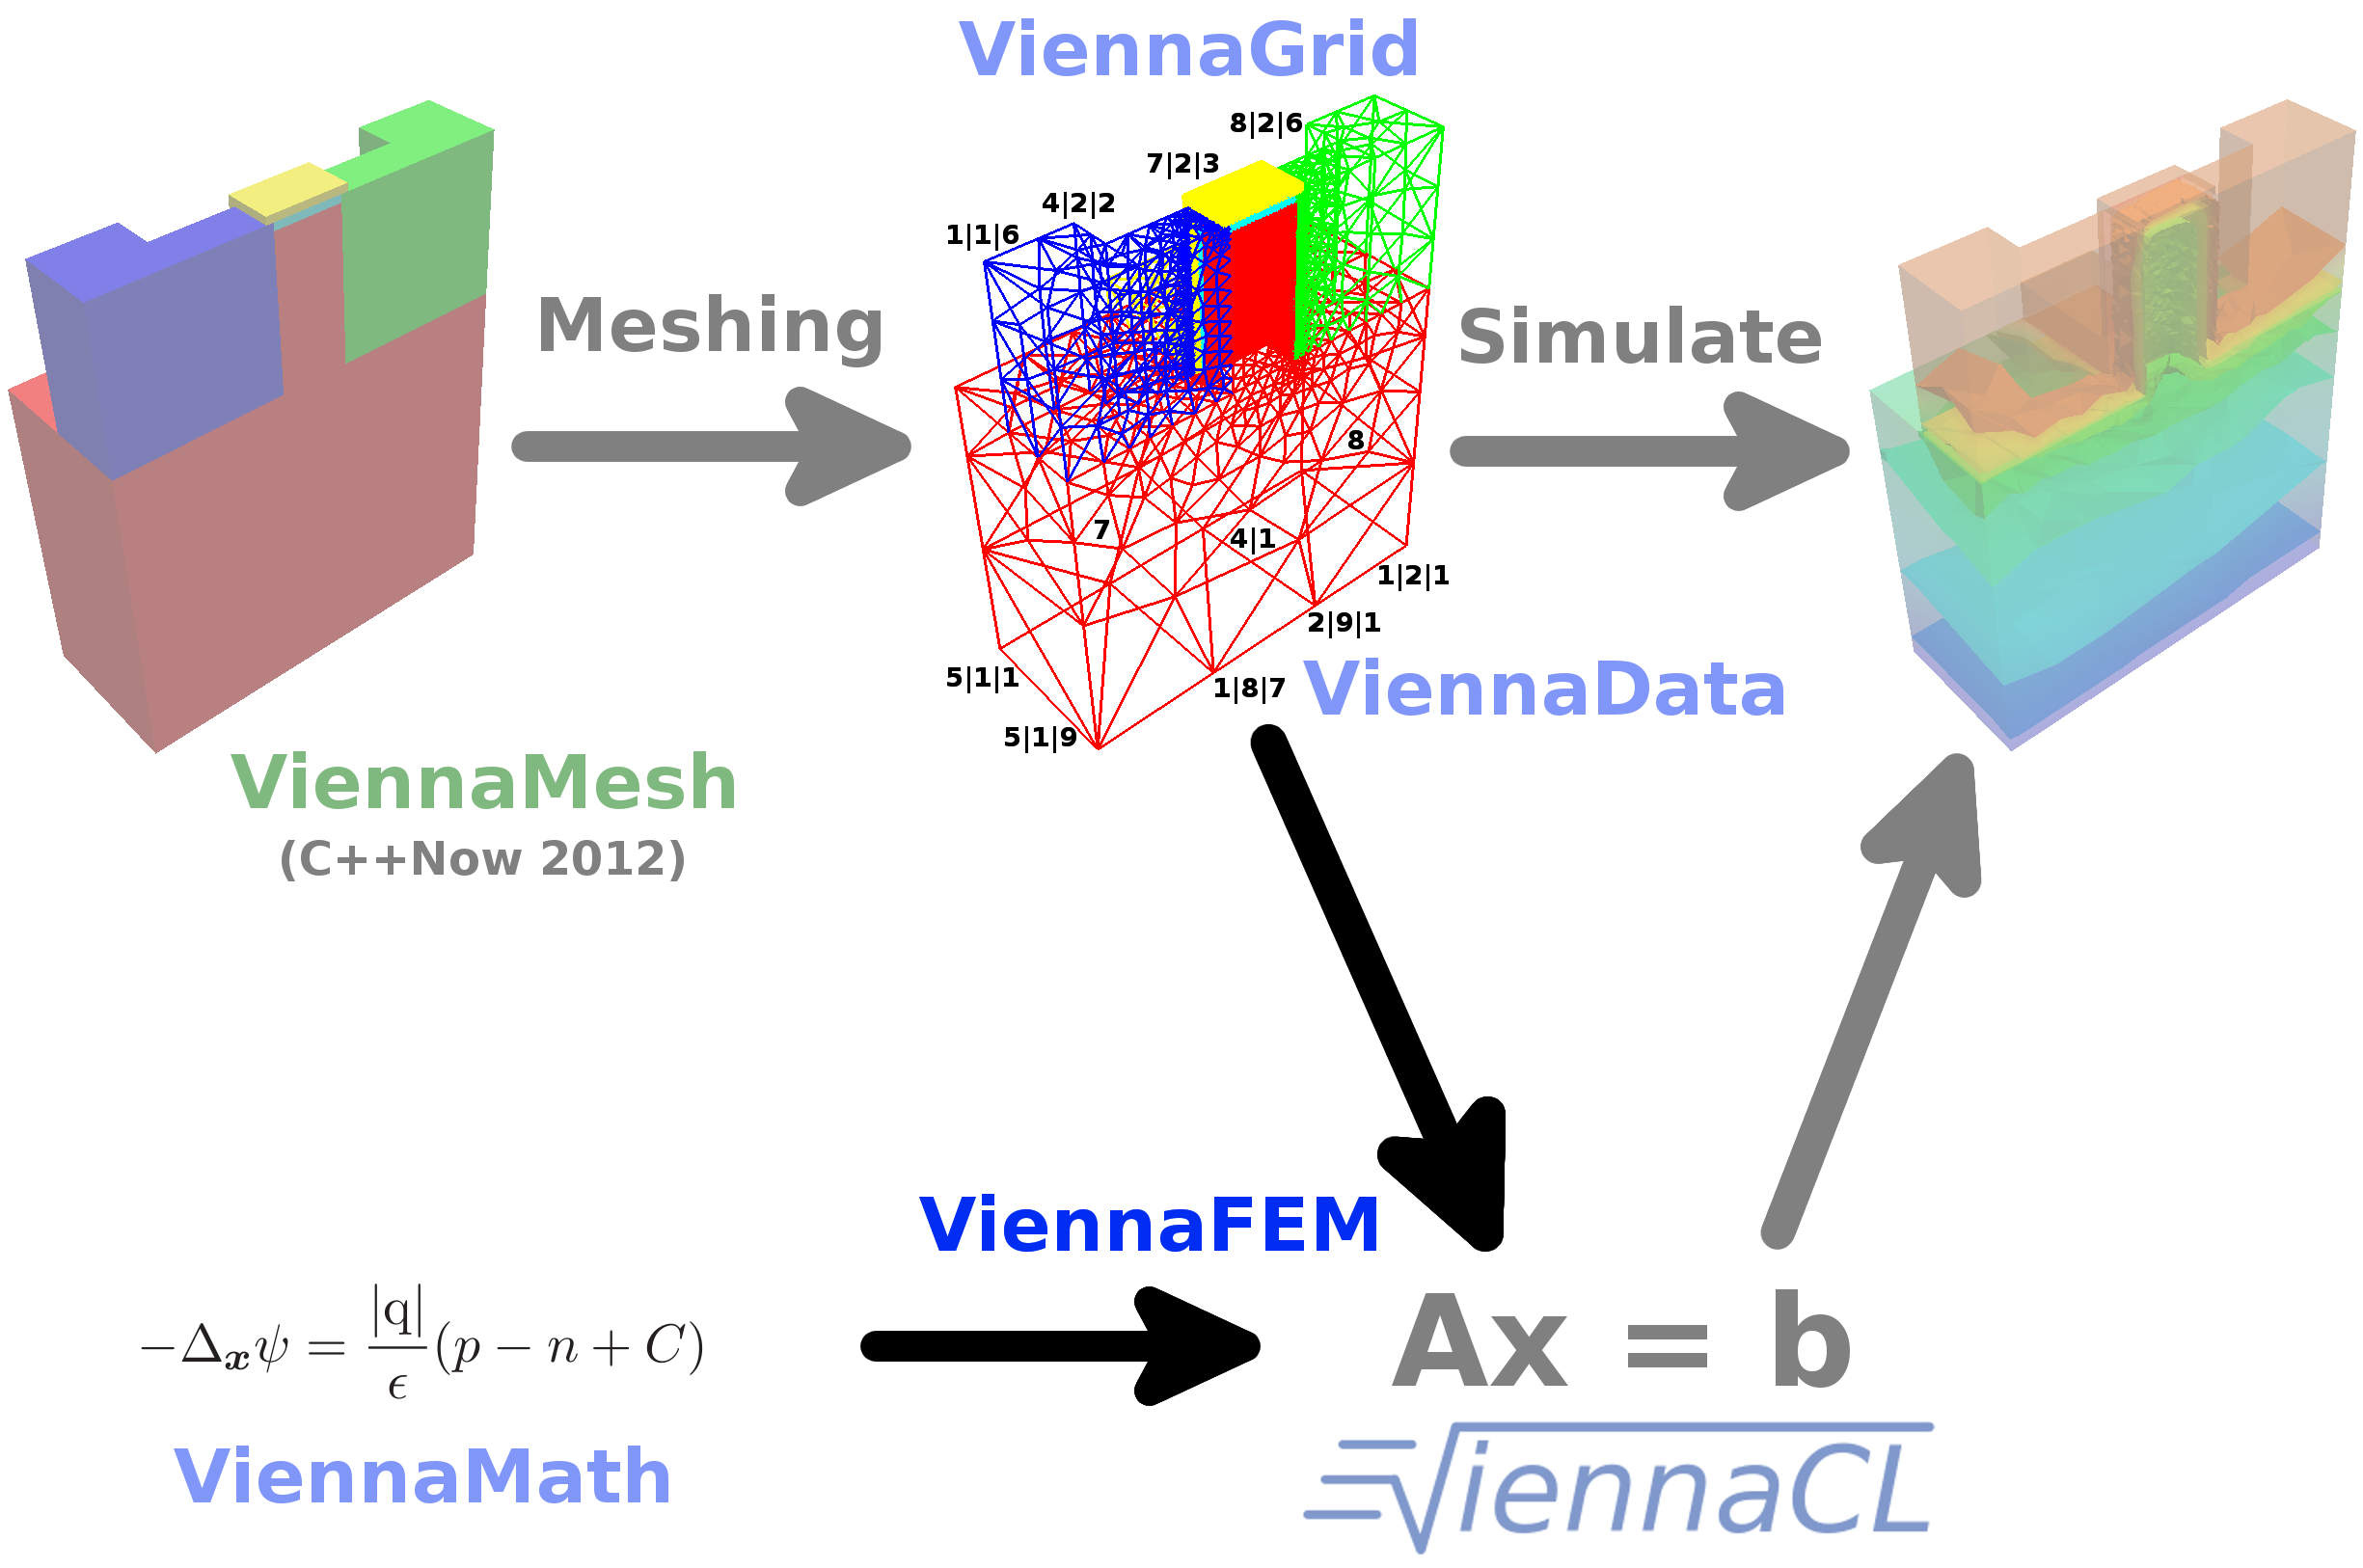
\includegraphics[width=0.99\textwidth]{flow-viennafem-2.png}
  \end{center}
\end{frame}


%%%%%% Expected talk time: 10 minutes, ~5 slides  (maybe with backup slides)


\begin{frame}{Simulation Flow}

  \begin{center}
   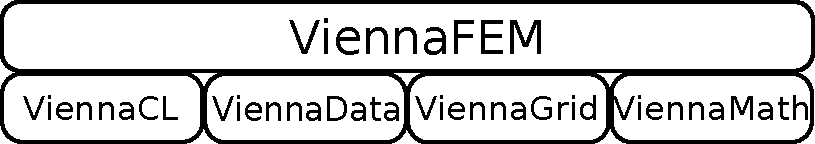
\includegraphics[width=0.6\textwidth]{ViennaFEM-arch.pdf}
  \end{center}
 \begin{block}{Library-Centric Design}
  \begin{itemize}
   \item ViennaCL for linear solver
   \item ViennaData for data storage
   \item ViennaGrid for mesh handling
   \item ViennaMath for symbolic math
  \end{itemize}
 \end{block}
 
 \visible<1->{
 \begin{block}{Addresses Come\&Go in Academia}
  \begin{itemize}
   \item Focus on one package
   \item No in-depth knowledge of all packages required
   \item Additional emphasis on good interfaces
  \end{itemize}
 \end{block}
 }
 
\end{frame}

%%%%%%%%%%%%%%%%%%%%%%%5



\begin{frame}[fragile]
\frametitle{ViennaFEM}

\begin{block}{ViennaGrid deals with the Mesh}
\begin{lstlisting}[basicstyle=\scriptsize\ttfamily]
DomainType my_domain;
viennagrid::io::netgen_reader my_reader;
my_reader(my_domain, "mystructure.mesh");
\end{lstlisting}
\end{block}

\begin{block}{Equation specification via ViennaMath: $\color{black} \Delta u = -1$}
\begin{lstlisting}[basicstyle=\scriptsize\ttfamily]
equation poisson_eq = viennamath::make_equation(laplace(u), -1);
\end{lstlisting}
\end{block}


\begin{block}{Assembly via ViennaFEM}
\begin{lstlisting}[basicstyle=\scriptsize\ttfamily]
viennafem::pde_assembler fem_assembler;
fem_assembler(viennafem::make_linear_pde_system(poisson_eq, u),
              my_domain,
              system_matrix, load_vector);
\end{lstlisting}
\end{block}

\begin{block}{Linear solver provided by ViennaCL}
\begin{lstlisting}[basicstyle=\scriptsize\ttfamily]
VectorType pde_result 
  = viennacl::linalg::solve(system_matrix, load_vector, cg_tag());
\end{lstlisting}
\end{block}
 
\end{frame}


%%%%%%%%%%%%%%%%%%%%%%%

\begin{frame}[fragile]
\frametitle{ViennaFEM}

 \begin{block}{Lame equation for Linear Elasticity}

  \begin{align*} 
    \int_\Omega \varepsilon(u) : \sigma(v) \: \mathrm{d} \Omega =
    \int_\Omega F \cdot v \: \mathrm{d} \Omega \quad \forall v \in \mathcal{V}
  \end{align*}

   \begin{itemize}
    \item With $F = (0, 0, 1)^{\mathrm{T}}$:
   \end{itemize}
   
  \begin{lstlisting}
  std::vector< Expression > strain = strain_tensor(u);
  std::vector< Expression > stress = stress_tensor(v);
  
  Equation weak_form_lame = make_equation(
             integral(symbolic_interval(),
                      tensor_reduce( strain, stress )),
             //=                                         
             integral(symbolic_interval(),
                      constant(1.0) * v[2])
                                         );
  \end{lstlisting}
   

 \end{block}

\end{frame}

\begin{frame}{Solving Lame's Equation for a TSV}
 \begin{center}
  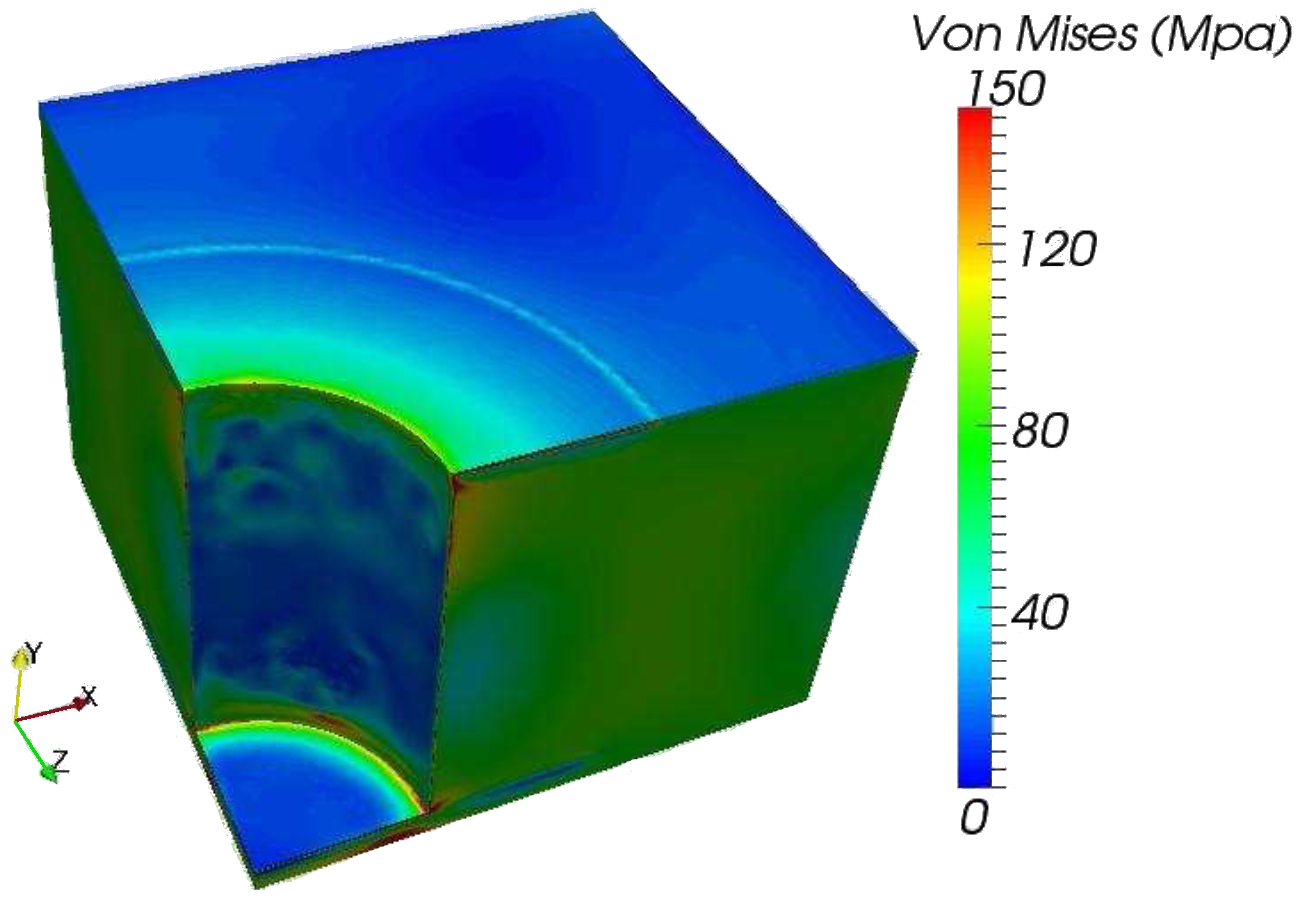
\includegraphics[width=0.8\textwidth]{figures/tsv.png}
 \end{center}
\end{frame}


